% !TEX encoding = UTF-8 Unicode
\documentclass[aodsor,preprint]{imsart}
\usepackage{amsthm,amsmath,amssymb}
\usepackage{graphicx}
%\usepackage[authoryear,round]{natbib}
\usepackage[
backend=biber,
natbib=true,
language = english,
doi = false, url = false, isbn = false, eprint = false,
style = apa]
{biblatex}
\DeclareLanguageMapping{english}{english-apa}
\addbibresource{sources.bib}
\usepackage[colorlinks,citecolor=blue,urlcolor=blue]{hyperref}
\usepackage[utf8]{inputenc}
\usepackage{relsize}
\usepackage{dsfont}
\usepackage{float}
\usepackage{hyperref}
\usepackage{xcolor}
%\usepackage{ngerman}


% settings
%\pubyear{2005}
%\volume{0}
%\issue{0}
%\firstpage{1}
%\lastpage{8}
%\arxiv{arXiv:0000.0000}


\numberwithin{equation}{section}
\theoremstyle{plain}
\newtheorem{thm}{Theorem}[section]
\newtheorem{lemma}[thm]{Lemma}
\newtheorem{corollary}[thm]{Corollary}
\newtheorem{remark}[thm]{Remark}
\newtheorem*{remark*}{Remark}

% customize math operators
\newcommand{\E}{{\mathbb E}}


\begin{document}

\begin{frontmatter}
\title{Scraping the Synthetic Risk and Reward Indicator from Funds' Key Information Documents}
\runtitle{Scraping Key Information Documents}

\begin{aug}
\author{\fnms{Fabian} \snm{Blasch}\ead[label=e1]{blasch57@gmail.com}}



%\runauthor{Fabian Blasch}

\affiliation{University of Vienna}

\end{aug}

\begin{abstract}
INSERT ABSTRACT
\end{abstract}

\begin{keyword}[class=MSC]
\kwd[Primary ]{Key1}
\kwd{Key2}
\kwd[; secondary ]{Key3}
\end{keyword}

\begin{keyword}
\kwd{Scraping}
\kwd{\LaTeXe}
\end{keyword}

\end{frontmatter}

\section{Introduction}
According to BGBl. II Nr. 265/2011, effective 2011, every undertaking for collective investment in transferable securities (UCITS), has to publish a key information document (KID)\citep{BGB1}. Said document is supposed to inform potential and current investors about various characteristics of the investments at hand. Besides a short description of the investments as well as performance measured against a benchmark, this document also contains a synthetic risk- and reward indicator (SRRI). As the name suggests, the purpose of this indicator is to measure the risk associated with an investment in the respective fund. How the SRRI is derived depends on the class of investment fund and will be described in greater detail in a separate subsection. Independent of the exact procedure of derivation the underlying interpretation of risk is measured via the volatility of returns.\\
The aim of this thesis is to firstly, give a short and precise introduction into the calculation of the SRRI.Then the data is briefly presented and the approach to measuring extraction performance is discussed. The following sections focus shifts to extracting the SRRI which is displayed as a graph, usually on the first page of every KID. The description of the extraction is based on pseudo-code which aims to aid the reader in understanding the approach taken to obtain the SRRI. In order to keep the structure as simple as possible the proccess is split into a parent function which calls a variety of helper functions.

\newpage

\section{SRRI}

The SRRI aims to measure risk via the volatility of weekly returns from the last 5 years, should weekly retuns be unobtainable, the calculation may be executed using montly returns.Accordingly, by ordinance the SRRI may be obtained as follows

\[
\sigma_f = \sqrt{\frac{m}{T - 1}\text{ }\mathlarger{\sum}_{t = 1}^{T} (r_{f, t} - \overline{r_f})^2},
\]

where $r_{f, t}$ is the fund's return and $\overline{r_f}$ represents the mean of returns over $T$ periods. Then scaling via  $m$, the return frequency within a year, yields the standard deviation of yearly returns. For illustrative purposes, the calculation using weekly returns would result in $m = 52$, as there are 52 months in a year and $T = 5 * 52 = 260$ the number of months in 5 years. To obtain the SRRI which is measured on a scale from 1 to 7 the regulating autorithy provides a table.
\begin{table}[H]
\begin{center}
	\caption{SRRI Classification}
\begin{tabular}{|c|c|c}
	\hline
	SRRI & $\sigma_f$ \\
	\hline
	1 & $0\% \leq\sigma_f<0.5\%$\\
	\hline
	2 & $0.5\%\leq\sigma_f<2\%$\\
	\hline
	3 & $2\%\leq\sigma_f<5\%$\\
	\hline
	4 & $5\%\leq\sigma_f<10\%$\\
	\hline
	5 & $10\%\leq\sigma_f<15\%$\\
	\hline
	6 & $15\%\leq\sigma_f<25\%$\\
	\hline
	7 & $25\%\geq\sigma_f$\\
	\hline
\end{tabular}
\end{center}
\end{table}

\section{Measuring Scraping Performance}

The SRRI is measured on an increasing ordinal scale, with 7 being associated with the highest risk and simultaneously also with the highest return. This would in theory allow for a measurement of predictive performance utilizing the abolute or squared difference between prediction and actual value. However, in this case we want to measure whether the read-out was successful or not. Hence the performance evaluation will be based on predicting correctly. Formally this means, we will use a discrete metric, i.e

\[
Accuracy = \frac{1}{n}\mathlarger{\sum}_{i = 1}^n\mathds{1}_{\{pred_i \text{ }= \text{ } act_i\}}\text{.}
\]

Put differently, the accuracy measure is equivalent to the relative amount of correctly predicted cases.
\newpage

\section{Data}
As previoulsy mentioned the KIDs are available to download from the respective fund managing firm. The sample used for measuring the extracting performance contains 121 Key Information documents, obtained from the websites of the respective KAG (Kapitalanlagegesellschaft). The distribution of the SRRI as well as the amount of KIDs per KAG within the sample are displayed below.

\begin{figure}[H]
	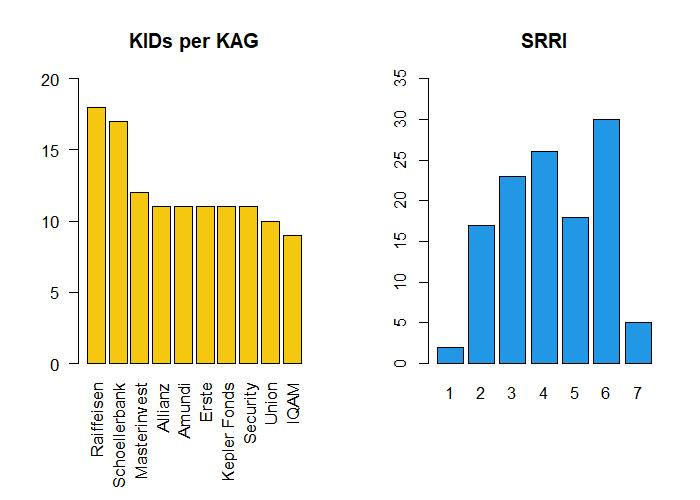
\includegraphics[width = 12cm]{data_overview}
	\caption{Number of KIDs per KAG and distribution of SRRI}
\end{figure}

The two depicted plots give a good impression of the sample at hand. We can immediately observe that two KAGs are overrepresented in the sample, namely Raiffeisen and Schoellerbank. Further, we can see that for the remaining fund managing firms around 10 KIDs are available in the sample. Regarding the distribution of the SRRI, the graph depicted on the right enables us to notice that the sample seems to contain very little funds that are associated with an SRRI of 1 or 7. The low number of funds classified into the first class may be due to the way the standard deviation of retrurns is converted into the SRRI. The intervals which are used to determin the SRRI increase in length quite signigicantly. The first interval for which $0\% \leq\sigma_f<0.5\%$ spans a range of half a percent, while the intervall for the classification into the 6th class $15\%\leq\sigma_f<25\%$ spans 10\%. The other end, namely the SRRI of 7, could be underrepresented because of a lack in demand for such high risk products. Of course this is just mere speculation but interesting nonetheless.\newpage
In regards to the extraction, to ease illustration of the coming chapters, an example document from Erste can be found \href{https://github.com/Base-R-Best-R/KID/blob/main/KIDs/Erste/kid-eb-147-t2957-at_de-de_en_4.pdf}{\textcolor{teal}{here}}. Additionally, an example of the SRRI graph as it can be found in an Erste KID is provided below.

\begin{figure}[H]
	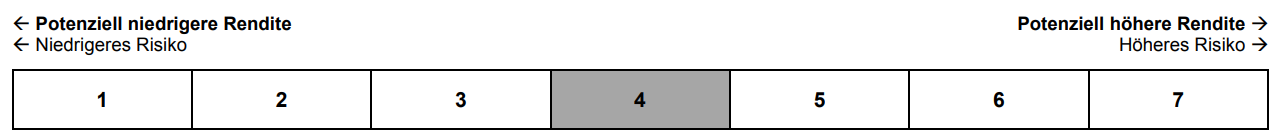
\includegraphics[width = 12cm]{example_SRRI_graph}
	\caption{Example of the SRRI graph from an Erste KID}
\end{figure}

\section{Naive Approach}

\section{Agglomerative Clustering}
\newpage
%========= Appendix ==========

\appendix


\section{Code}
\label{sec:app}

Appendix for code and additional illustrations

\subsection{Functions}




%====== References ========


\newpage
\printbibliography


\end{document}
